\section{Fonctionnalités}
Une des limitations du ray marching est que l'on ne peut pas mettre n'importe quel objet 3D dans la scène.\\
En effet, nous sommes limités aux objets 3D pour lesquels existent une Signed Distance Function (SDF). C'est ce que l'on appellera volumes élémentaires. On peut ensuite combiner ces objets, soustraire leurs volumes, appliquer des transformation pour obtenir de nouveaux objets.

\subsection{Volumes élémentaires}
Dans cette partie, on s'intéresse aux fonctions Signed Distance Function (SDF) de différentes formes géométriques. On remarque que toutes ces fonctions supposent que l'objet géometrique est centré en $O$. Cela simplifie beaucoup les fontions et il est très facile de leur appliquer une translation ou autre transformation, comme indiqué dans \ref{subsec:Transformations} \nameref{subsec:Transformations}.
\subsubsection{Sphère}
La sphere a la plus simple des SDF. En effet, la distance entre un point $P$ et une sphere de rayon $r$ est donnée par 
\begin{align*}
distance=length(P)-r
\end{align*}
Avec $length(x)=\|x\|_2$.
\\\textbf{Remarque:} On rappelle que le volume est centré en O.
\subsubsection{Plan}
La distance entre un point $P$ et un plan de normale $N$ (normalisée) et de hauteur $h$ est donnée par 
\begin{alignat*}{1}
    distance=\left\langle P,N \right\rangle - h
\end{alignat*}
\subsubsection{Et bien d'autres\ldots}
Il existe de nombreuses autres fonctions SDF. Cependant, elles deviennent très vite complexes à comprendre.\\
Voici par exemple la fonction SDF pour un pavé avec $taille=(largeur, hauteur, profondeur) \in \mathbb{R}^3$
Cette fontion utilise le fait que la fonction |.| sur un vecteur équivaut à une symétrie par rapport aux plans xOy, xOz et yOz. Or, un pavé centré en O possede ces trois plans de symétries. Ainsi, la distance d'un point $P$ à ce pavé est donnée par le code suivant:

\begin{lstlisting}[language=GLSL]
float SDF_Box(vec3 p, vec3 taille) {
	vec3 q=abs(p)-taille;
	return length(max(q,0.0))+ min(max(q.x,max(q.y,q.z)),0.0);
}
\end{lstlisting}
\newpage
\subsection{Transformations}\label{subsec:Transformations}
Les transformations sont une des spécificités la plus utile et unique du $Ray\ Marching$. En effet, elles sont extremement peu couteuses en ressources, et permettent de creer des formes uniques.
\\Pour toutes transformations il suffit, lorsqu'on veut obtenir la distance entre un point $P$ de l'espace et un objet transformé, de prendre la distance entre la \textbf{transformation inverse} du point $P$ et l'objet non transformé.
\\
\begin{align*}
    SDF\_Objet\_Tranforme(P)=SDF\_Objet(Transformation\_Inverse(P))
\end{align*}
Nous allons maintenant voir quelques exemples.

\subsubsection{Translation}
Pour obtenir une translation de vecteur $translation$ d'un objet, on peut utiliser le code suivant :
\begin{lstlisting}[language=GLSL]
SDL_Objet(p-translation);
\end{lstlisting}

\subsubsection{Rotation autour des axes XYZ}
Pour une rotation autour des axes X, Y et Z, d'angles respectivement $alpha$, $beta$ et $gamma$ d'un objet, on utilise le code suivant:
\begin{lstlisting}[language=GLSL]
SDL_Objet(Rotation(p,-alpha,-beta,-gamma))
\end{lstlisting}
Avec $Rotation$ une application linéaire dont la matrice dans la base cannonique est donnée ici : 
\begin{align*}
    R(x,y,z)
    =& R_{ex}(x)R_{ey}(y)R_{ez}(z) \\
    = &
    \begin{bmatrix}
    cos(x) & -sin(x) & 0 \\
    sin(x) & cos(x) & 0 \\
    0 & 0 & 1 
    \end{bmatrix}
    \begin{bmatrix}
    cos(y) & 0 & sin(y) \\
    0 & 1 & 0 \\
    -sin(y) & 0 & cos(y) 
    \end{bmatrix}
    \begin{bmatrix}
    1 & 0 & 0 \\
    0 & cos(z) & -sin(z) \\
    0 & sin(z) & cos(z) 
    \end{bmatrix}\\
    = & \begin{bmatrix}
    cos(y)cos(z) & sin(x)sin(y)cos(z) & cos(x)sin(y)cos(z)+sin(x)sin(z) \\
    cos(y)sin(z) & sin(x)sin(y)sin(z)+cos(x)cos(z) & cos(x)sin(y)sin(z)-sin(x)cos(z) \\
    -sin(y) & sin(x)cos(y) & cos(x)cos(y)
    \end{bmatrix} \\
\end{align*}

\subsubsection{Duplication des volumes}
Il est egalement possible d'appliquer des transformations plus complexes, permettant par exemple de dupliquer des objets.
\\Pour dupliquer un nombre infini de fois un volume, il suffit d'appliquer un modulo (reste de la division entière) sur la position de l'objet.
\\Le code pour dupliquer un objets à l'infini sur l'axe Ox, toutes les $N$ unités, est celui-ci:
\begin{lstlisting}[language=GLSL]
SDF_Objet( vec3( mod(p.x - N/2, N) + N/2, p.y, p.z))
\end{lstlisting}
\textbf{Remarque:} $vec3$ est un constructeur de vecteur 3D

\newpage
\subsubsection{symétrie}
Il est egalement possible de faire des symetrie par rapport à une plan de normale $N$ et de décalage $offset$. Le code est le suivant:
\begin{lstlisting}[language=GLSL]
SDF_Objet(symetrie(p,-normale,-offset));
\end{lstlisting}
Avec le code de $symetrie$ :
\begin{lstlisting}[language=GLSL]
vec3 symetrie(vec3 position, vec3 normale,float offset){
    float d=dot(position,normale) + offset;
    if (d>0) return position;
    else return position-2.0*d*normale;
}
\end{lstlisting}
Avec $dot$ le produit scalaire.
\\\textbf{Remarque:} Cette symetrie ne fonctionne que dans un seul sens. C'est à dire que l'un des coté du plan "disparait" pour laisser place au symetrique de l'autre coté du plan.
\subsection{Vue orthogonale et perspective}
Le moteur graphique permet de changer de mode de vue et permet de passer d'une vue en perspective (active par défaut) à une vue orthogonale.\\
Cette vue est très utilisée notamment dans les logiciels de modélisation 3D mécanique.\\
\par
Pour obtenir cette vue, il suffit d'assigner la position de la caméra comme étant la position de l'écran et d'affecter $e_z$ (la direction de la caméra) aux vecteurs des pixels de l'écran à l'écran.
\begin{figure}[h]
    \centering
    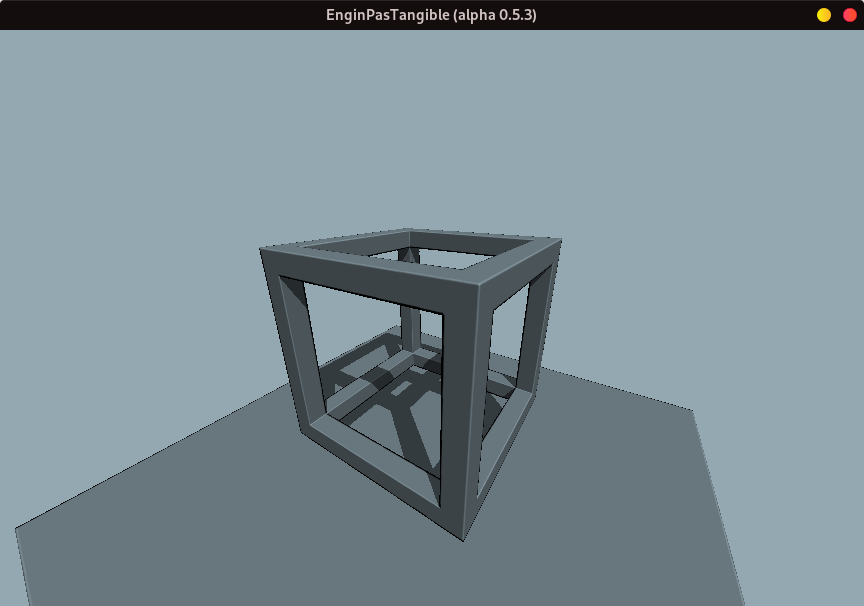
\includegraphics[width=7cm]{images/screens/orthoff.png}
    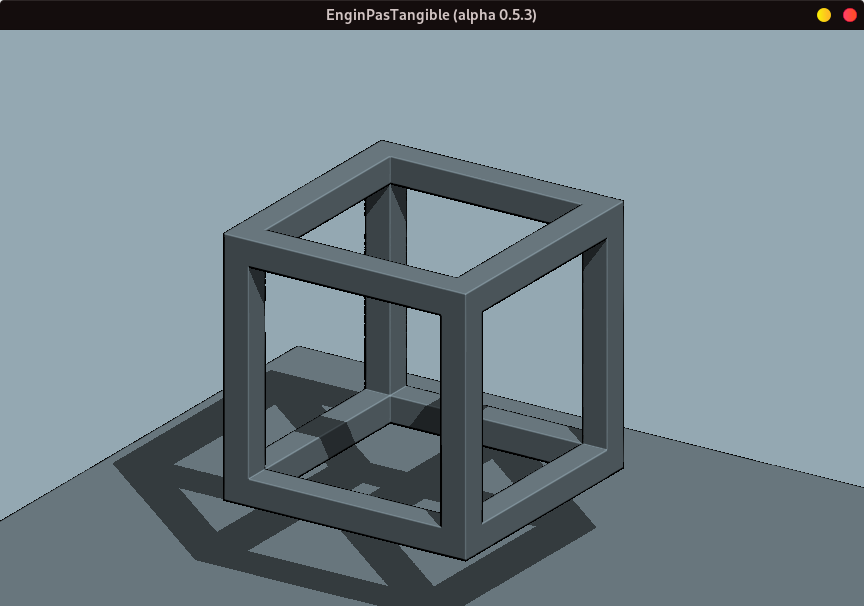
\includegraphics[width=7cm]{images/screens/orthon.png}
    \caption{Différence entre perspective et vue orthogonale}
    \label{fig:ombres}
\end{figure}